\documentclass[12pt]{scrartcl}

% packages
\usepackage[
    a4paper, total={18cm, 26cm},
    left=0.75in,
    right=0.75in,
    top=0.75in,
    bottom=0.50in,
    footskip=15pt
]{geometry}
\usepackage{lastpage}
\usepackage{graphicx} % \includegraphics
\usepackage{amsmath, esint} % math
\usepackage{steinmetz} % \phase
\usepackage{import} % \import
\usepackage{esdiff} % \diff
\usepackage{fancyhdr} % header and footer
\usepackage{listings}

\makeatletter
\def\today{%
  \two@digits{\the\day}/%
  \ifcase\month\or%
  01\or 02\or 03\or 04\or 05\or 06\or%
  07\or 08\or 09\or 10\or 11\or 12\fi/%
  \number\year%
}
\makeatother

% configs
\setlength{\parindent}{0pt}

% comandos
\renewcommand{\familydefault}{\sfdefault}
\newcommand{\un}[1]{\;\textrm{#1}}
\newcommand{\logo}{\quad \Rightarrow \quad}
\newcommand{\fase}[1]{\ensuremath{\phase{{#1}^{\circ}}}}

\newcommand*\VF[1]{\mathbf{#1}}
\newcommand*\dif{\mathop{}\!\mathrm{d}}


\begin{document}

\pagestyle{fancy}

\fancyhead{}
\fancyhead[L]{Python Aplicado a Sinais e Sistemas - PET Engenharias}
\fancyhead[R]{Data: \today}
\fancyfoot{}
\fancyfoot[R]{Pág. \thepage \; / \pageref{LastPage}}

\begin{center}
    Aluno: Raphael Henrique Braga Leivas \\[20pt]
    Email: rapha.lei8@gmail.com
\end{center}

\hrule

\section*{Atividade 2 - Capítulo 3}

O código completo usado nessa atividade se encontra no ANEXO A.

\subsection*{Exercício 1 (a)}

Temos um sistema linear dado por

\[  - 4 y{\left(t \right)} + 3 \frac{d}{d t} y{\left(t \right)} + \frac{d^{2}}{d t^{2}} y{\left(t \right)} = - 2 x{\left(t \right)} + \frac{d}{d t} x{\left(t \right)} \]

e condições iniciais $y(0) = 8$ e $y'(0) = -2$.

Queremos saber a resposta à entrada zero. Para isso, fazemos $x(t)=0$, obtendo

\[  - 4 y{\left(t \right)} + 3 \frac{d}{d t} y{\left(t \right)} + \frac{d^{2}}{d t^{2}} y{\left(t \right)} =  0 \]

Que é uma EDO linear homogênea de segunda ordem. A solução $y(t)$ é obtida via a equação 
característica

\[ \lambda^{2} + 3 \lambda - 4 = 0 \]

Com raízes $\lambda_1 = -4$ e $\lambda_2 = 1$. Como as raízes são reais e distintas,
a solução é da forma

\[ y(t) = c_1 e^{\lambda_1 t} + c_2 e^{\lambda_2 t} \]

Usando as condições iniciais, obtemos

\[ y(t) = 6 e^{t} + 2 e^{- 4 t} \]

Com forma de onda mostrada abaixo:

\begin{figure}[h!]
	\begin{center}
    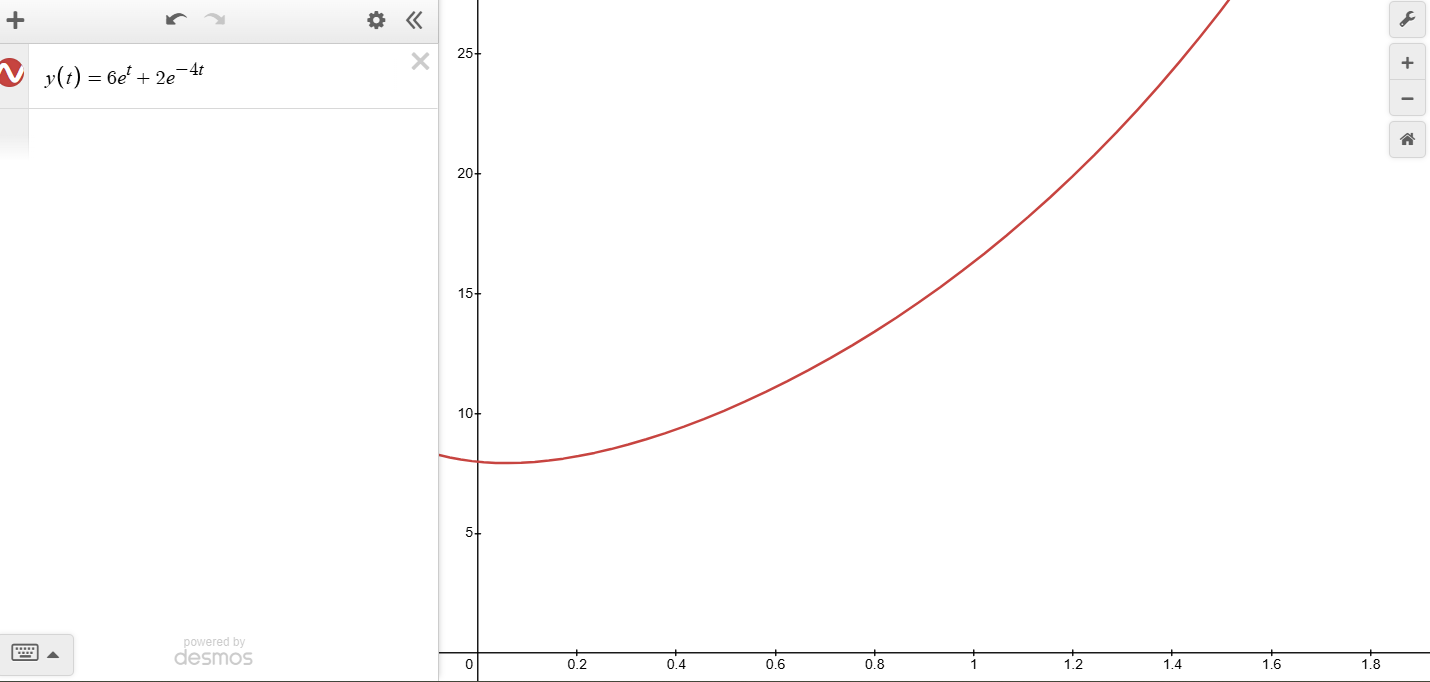
\includegraphics[width=0.8\textwidth,trim=1 1 1 1,clip]{ativ2-1a.png}
	\end{center}
\end{figure}

\subsection*{Exercício 1 (b)}

Temos um sistema linear dado por

\[  9 y{\left(t \right)} + 6 \frac{d}{d t} y{\left(t \right)} + \frac{d^{2}}{d t^{2}} y{\left(t \right)} = 7 x{\left(t \right)} + 2 \frac{d}{d t} x{\left(t \right)} \]

e condições iniciais $y(0) = 7$ e $y'(0) = -1$.

Usando o mesmo procedimento do item 1 (a), obtemos 

\[  9 y{\left(t \right)} + 6 \frac{d}{d t} y{\left(t \right)} + \frac{d^{2}}{d t^{2}} y{\left(t \right)} =  0 \]

\[ \lambda^{2} + 6 \lambda + 9 \]

Com apenas uma solução real $\lambda = -3$. Assim, a solução é da forma 

\[ y(t) = \left( c_1 + c_2 \right) e^{\lambda t}  \]

\[ y(t) = 8 t e^{- 3 t} + 3 e^{- 3 t} \]

\begin{figure}[h!]
	\begin{center}
    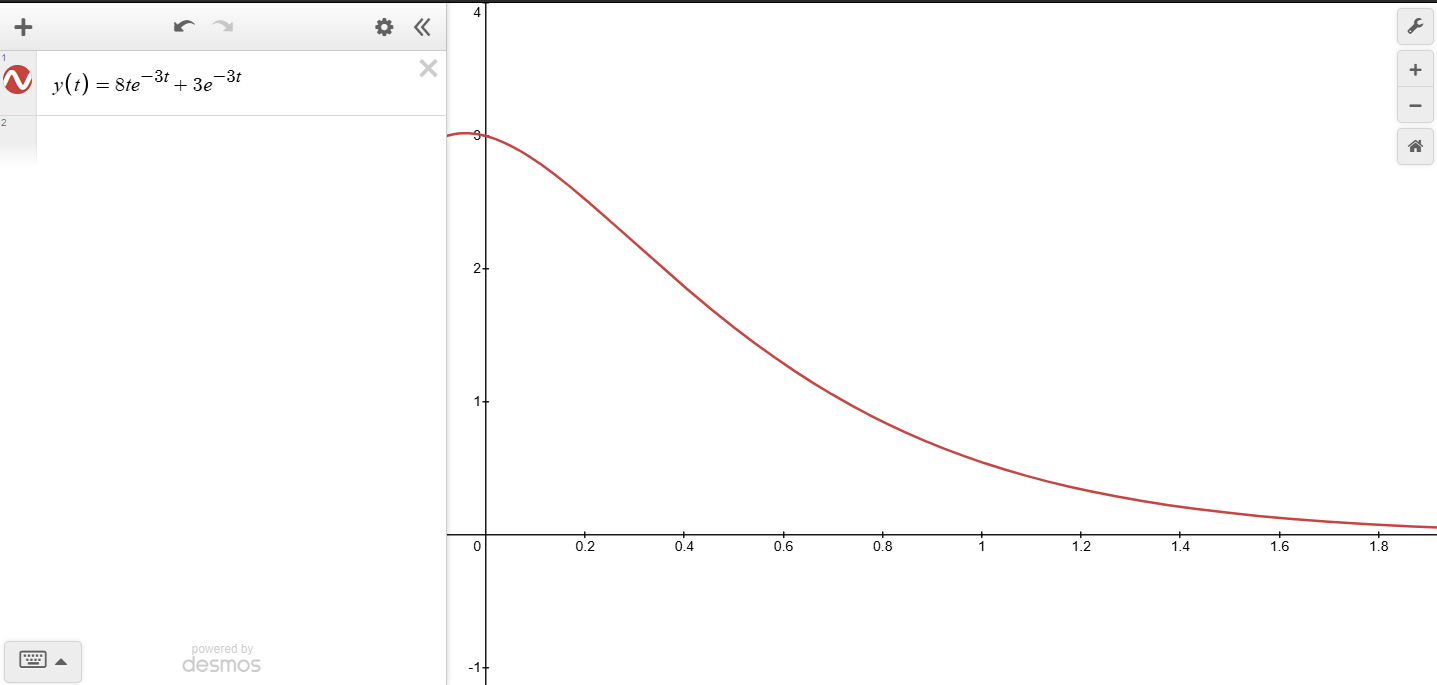
\includegraphics[width=0.8\textwidth,trim=1 1 1 1,clip]{ativ2-1b.png}
	\end{center}
\end{figure}

\subsection*{Exercício 2 (a)}

O sistema linear é definido por 

\[ 2 y{\left(t \right)} + 3 \frac{d}{d t} y{\left(t \right)} + \frac{d^{2}}{d t^{2}} y{\left(t \right)} = 2 x{\left(t \right)} + 3 \frac{d}{d t} x{\left(t \right)} \]

Tornando todas condições iniciais nulas e aplicando a Transformada de Laplace dos dois lados da equação, obtemos 

\[ 2 Y(s) + 3 s Y(s) + s^2 Y(s) = 2 X(s) + 3sX(s) \] 

\[ Y(s) \left(2 + 3s + s^2\right) = X(s) \left(2 + 3s\right) \] 

\[ H(s) = \frac{P_s}{Q_s} = \frac{Y(s)}{X(s)} = \frac{2 + 3s}{2 + 3s + s^2}\] 

Usando o software para tirar a transformada inversa, temos  

\[ h(t) = - e^{- t} + 4 e^{- 2 t} \]

\subsection*{Exercício 2 (b)}

Usamos o mesmo procedimento do item 2 (a). O sistema linear é definido por 

\[ - 4 y{\left(t \right)} + 3 \frac{d}{d t} y{\left(t \right)} + \frac{d^{2}}{d t^{2}} y{\left(t \right)} = - 2 x{\left(t \right)} + \frac{d^{2}}{d t^{2}} x{\left(t \right)} \]

\[ - 4 Y(s) + 3 s Y(s) + s^2Y(s) = -2X(s) + s^2X(s) \]

\[ H(s) = \frac{P_s}{Q_s} = \frac{Y(s)}{X(s)} = \frac{-2 + s^2}{4 + 3s + s^2}\] 

Como os graus dos polinômios são iguais, temos que incluir o Delta de Dirac:

\[ h(t) = - \frac{e^{t}}{5} + 1 \delta (t) - \frac{14 e^{- 4 t}}{5} \]

\subsection*{Exercício 3 (a)}

A resposta ao estado nulo é definida por 

\[  y(t) = \int_{-\infty}^{-\infty} x(\tau) h(t - \tau) \,d\tau \]

No exercício, temos 

\[ x(\tau) = 500 \quad , \quad h(t - \tau) = e^{-(t - \tau)} - e^{-2(t - \tau)} \]

Resolvendo a integração de convolução com o software, temos

\[ y(t) = 250 - 500 e^{- t} + 250 e^{- 2 t} \]

\[ y(1) = 99.8941002234320 \]

\subsection*{Exercício 3 (b)}

Mesmo procedimento do item 3 (a). 

\[ x(\tau) = e^{\tau} \quad , \quad h(t - \tau) = 3 e^{-6(t - \tau)} + e^{(t - \tau)} \]

\[ y(t) = - \frac{\left(7 e^{6 t} + 6 e^{t}\right) e^{- 7 t}}{14} + \frac{13 e^{t}}{14} \]

\[ y(1) = 2.33911679776482 \]

\newpage

\section*{ANEXO A - Código}

\begin{lstlisting}[language=Python, breaklines=true, basicstyle=\scriptsize]
    from sympy import *

    ## Exercicio 1

    t = symbols('t')
    y = Function('y')(t)
    x = Function('x')(t)

    QN_coeffs = [9, 6, 1]
    PN_coeffs = [7, 2]
    cond_iniciais = [3, -1]

    # define a EDO
    edo_y = sum(coeff * Derivative(y, t, n) for n, coeff in enumerate(QN_coeffs))
    edo_x = sum(coeff * Derivative(x, t, n) for n, coeff in enumerate(PN_coeffs))
    edo_completa = Eq(edo_y, edo_x)
    print(latex(edo_completa))

    eq_homog = Eq(edo_y, 0) #x(t) = 0, entrada zero

    # edo linear homogenea de segunda ordem: resolve com polinomio caracteristico
    lambda_ = symbols('lambda')
    eq_carac = sum(coeff * lambda_**n for n, coeff in enumerate(QN_coeffs))
    print(latex(eq_carac))
    raizes = solve(eq_carac, lambda_)
    print(raizes)

    # analisa as raizes da eq caracteristica para montar a solucao geral
    sol_geral = 0
    constantes = []
    c_counter = 1

    raizes_mult = roots(eq_carac, lambda_)
    for raiz, mult in raizes_mult.items():
        for m in range(mult):
            constante = symbols(f'c{c_counter}')
            constantes.append(constante)
            sol_geral += constante * t**m * exp(raiz * t)
            c_counter += 1


    # cond iniciais
    condicoes = []
    for ordem, valor in enumerate(cond_iniciais):
        condicoes.append(Eq(sol_geral.diff(t, ordem).subs(t, 0), valor))

    sistema_equacoes = []
    for cond in condicoes:
        sistema_equacoes.append(cond.lhs - cond.rhs)

    solucao_sistema = solve(sistema_equacoes, constantes)

    solucao_final = sol_geral.subs(solucao_sistema)

    print(latex(solucao_final))

    ## Exercicio 2

    def resposta_ao_impulso(Ps, Qs):
        t = symbols('t', real=True, positive=True)
        s = symbols('s')

        Hs = Ps / Qs

        h_t = inverse_laplace_transform(Hs, s, t)

        return h_t

    s = symbols('s')

    QN_coeffs = [-4, 3, 1]
    PN_coeffs = [-2, 0, 1]
    edo_y = sum(coeff * Derivative(y, t, n) for n, coeff in enumerate(QN_coeffs))
    edo_x = sum(coeff * Derivative(x, t, n) for n, coeff in enumerate(PN_coeffs))
    edo_completa = Eq(edo_y, edo_x)
    print(latex(edo_completa))

    Qs = -4 + 3*s + s**2
    Ps = -2 + s**2

    h_t = resposta_ao_impulso(Ps, Qs)

    # verifica se e instantaneo
    grau_p = degree(Ps, s)
    grau_q = degree(Qs, s)

    if grau_p == grau_q:
        b_0 = LC(Ps, s)
        a_0 = LC(Qs, s)

        termo_dirac = b_0 / a_0
        print(latex(termo_dirac + h_t))
    else:
        print(latex(h_t))

    ## Exercicio 3
\end{lstlisting}



\end{document}